\documentclass[pdflatex,compress]{beamer}

%\usetheme[dark,framenumber,totalframenumber]{ElektroITK}
\usetheme[darktitle,framenumber,totalframenumber]{ElektroITK}

\usepackage{graphicx}

\title{PEMODELAN JARINGAN KOMUNIKASI}
\subtitle{OSI Layer 3 - The Network Layer}

\author{Mifta Nur Farid, S.T., M.T.}

\begin{document}

\maketitle

\section{The IP Header}

\begin{frame}
	\frametitle{Layer 3 – The Network Layer}
	\begin{itemize}
		\item The Network layer is responsible for routing packets to their destination and for Quality of Service.
		\item IP (Internet Protocol) is the best known Layer 3 protocol. IPv4 is the focus of this section.
		\item It is a connectionless protocol with no acknowledgements at Layer 3.
		\item Other Layer 3 protocols include ICMP (Internet Control Message Protocol) and IPSec.
	\end{itemize}
\end{frame}

\begin{frame}
	\frametitle{IP Addressing}
	\begin{itemize}
		\item IP addressing is a logical addressing scheme which is implemented at Layer 3.
		\item The network designer uses IP addressing to partition the overall network into smaller ‘subnets’.
		\item This improves performance and security and makes troubleshooting easier.
		\item Layer 2 MAC addresses use one big flat addressing scheme. There is no logical separation between networks at Layer 2, it’s done at Layer 3.
	\end{itemize}
\end{frame}

\begin{frame}
	\frametitle{OSI Reference Model - Encapsulation}
	\begin{center}
		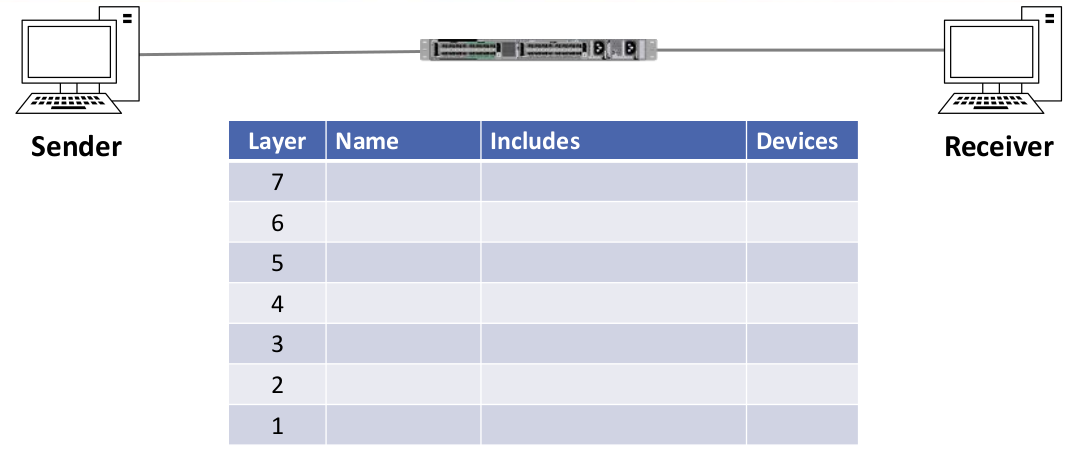
\includegraphics[width=\linewidth]{img/img01}
	\end{center}
\end{frame}

\begin{frame}
	\frametitle{OSI Reference Model - Encapsulation}
	\begin{center}
		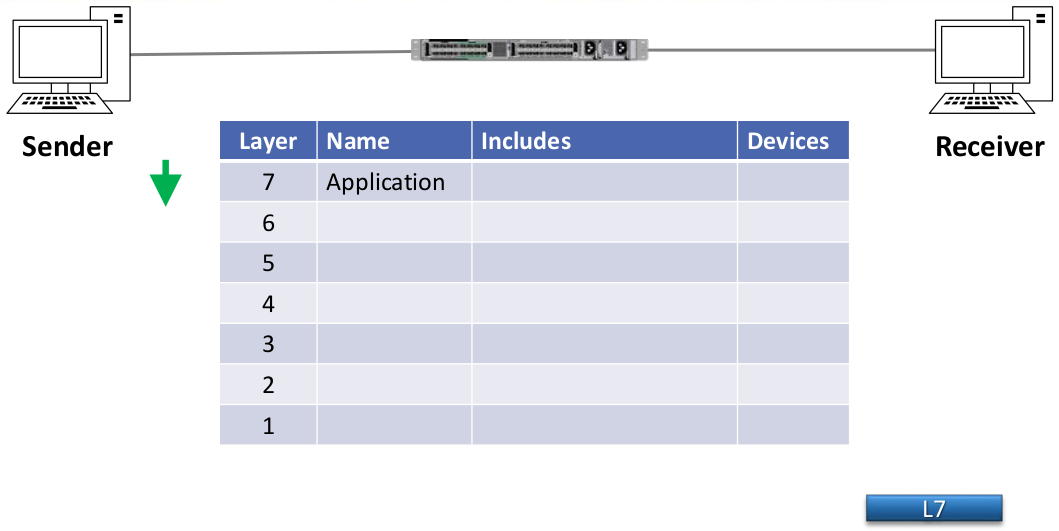
\includegraphics[width=\linewidth]{img/img02}
	\end{center}
\end{frame}

\begin{frame}
	\frametitle{OSI Reference Model - Encapsulation}
	\begin{center}
		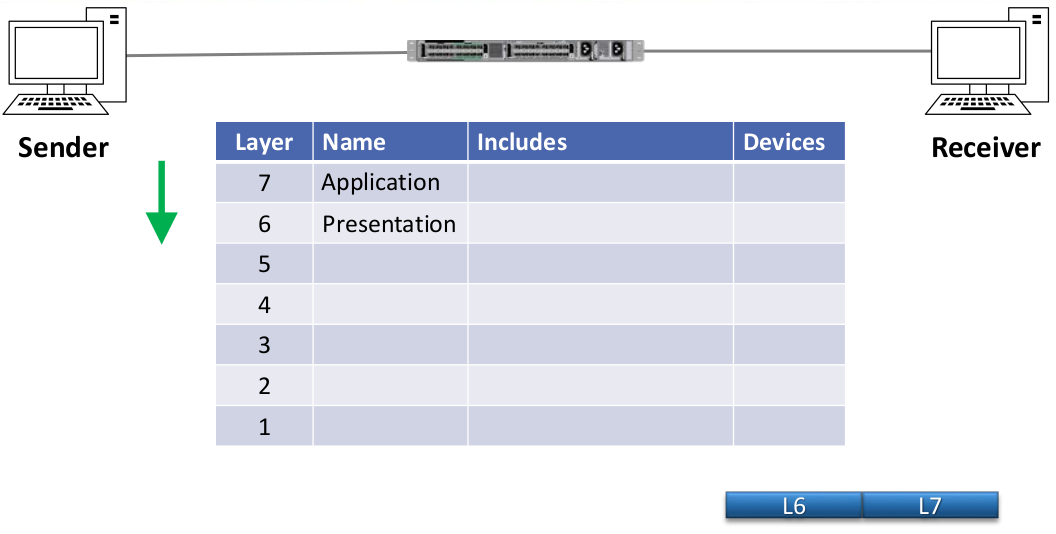
\includegraphics[width=\linewidth]{img/img03}
	\end{center}
\end{frame}

\begin{frame}
	\frametitle{OSI Reference Model - Encapsulation}
	\begin{center}
		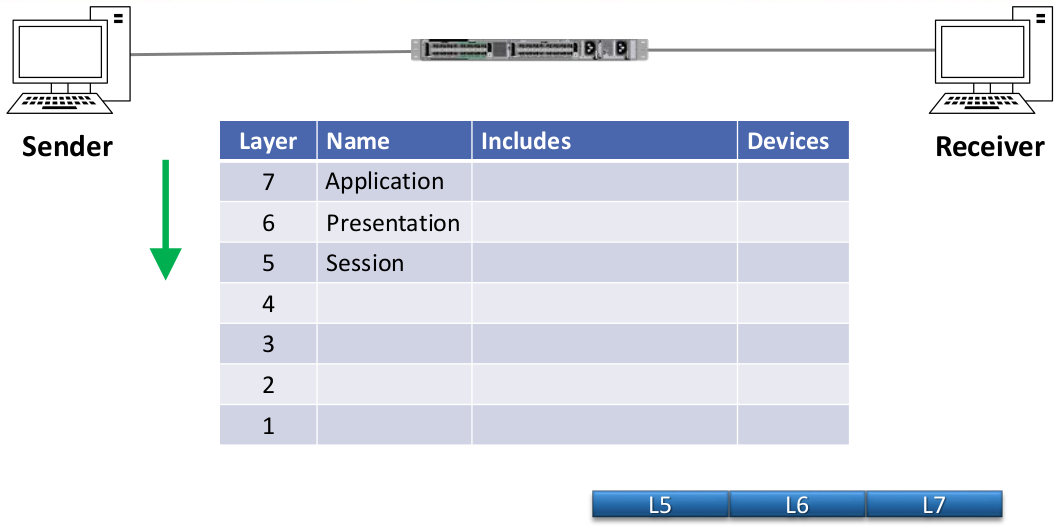
\includegraphics[width=\linewidth]{img/img04}
	\end{center}
\end{frame}

\begin{frame}
	\frametitle{OSI Reference Model - Encapsulation}
	\begin{center}
		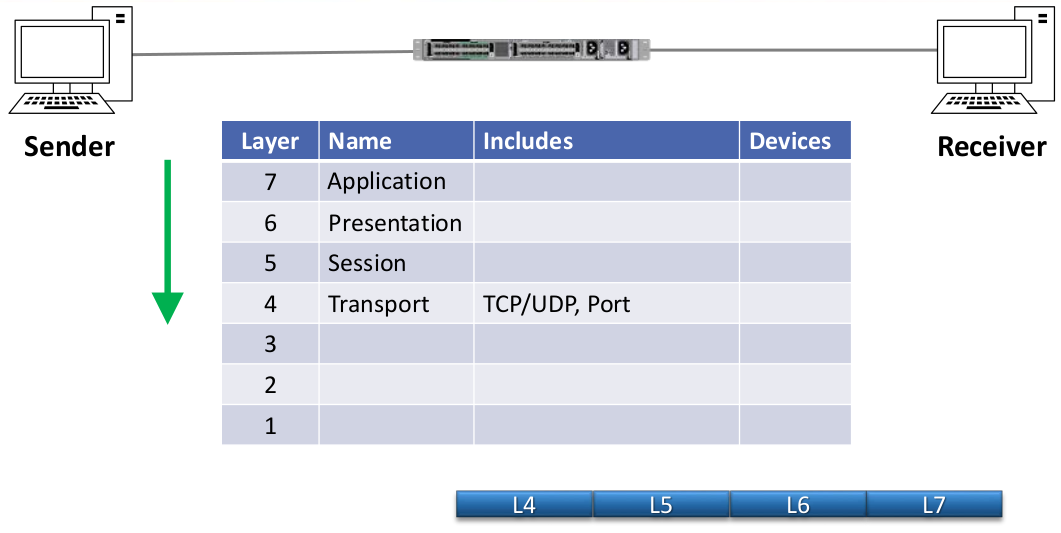
\includegraphics[width=\linewidth]{img/img05}
	\end{center}
\end{frame}

\begin{frame}
	\frametitle{OSI Reference Model - Encapsulation}
	\begin{center}
		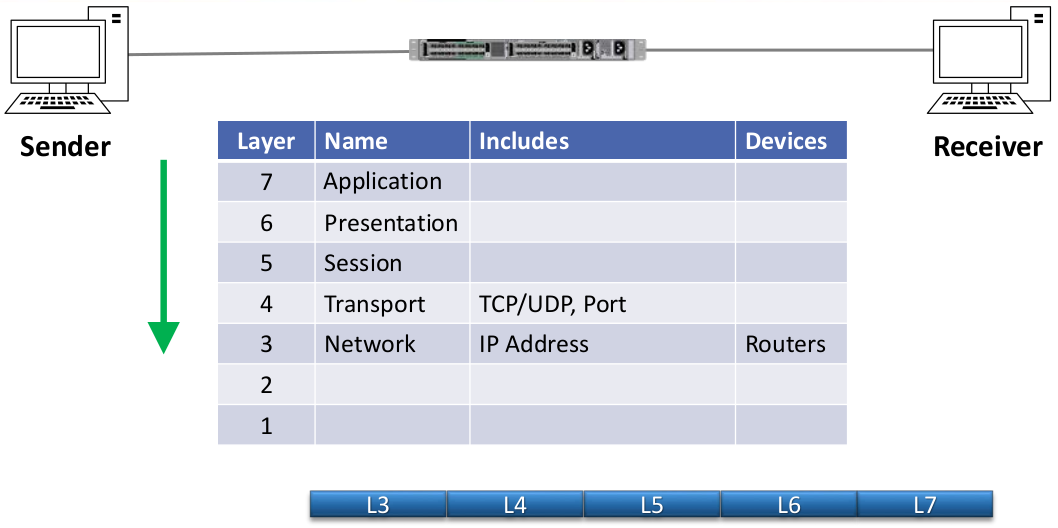
\includegraphics[width=\linewidth]{img/img06}
	\end{center}
\end{frame}

\begin{frame}
	\frametitle{OSI Reference Model - Encapsulation}
	\begin{center}
		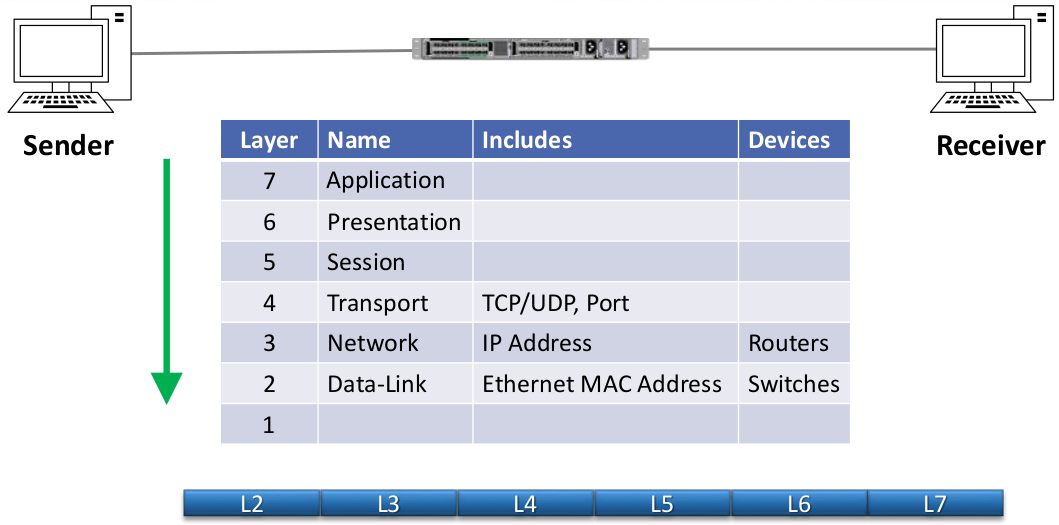
\includegraphics[width=\linewidth]{img/img07}
	\end{center}
\end{frame}

\begin{frame}
	\frametitle{OSI Reference Model - Encapsulation}
	\begin{center}
		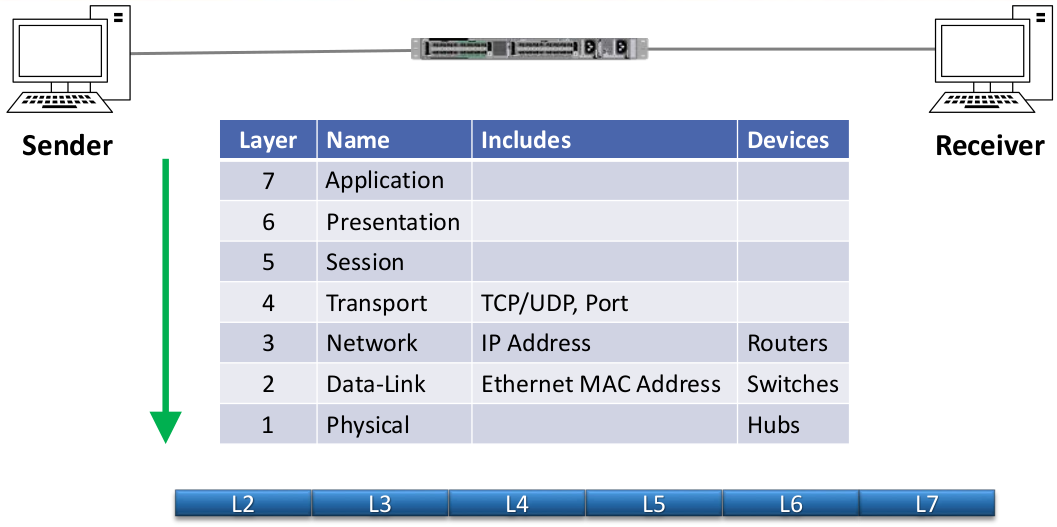
\includegraphics[width=\linewidth]{img/img08}
	\end{center}
\end{frame}

\begin{frame}
	\frametitle{The IP Header}
	\begin{center}
		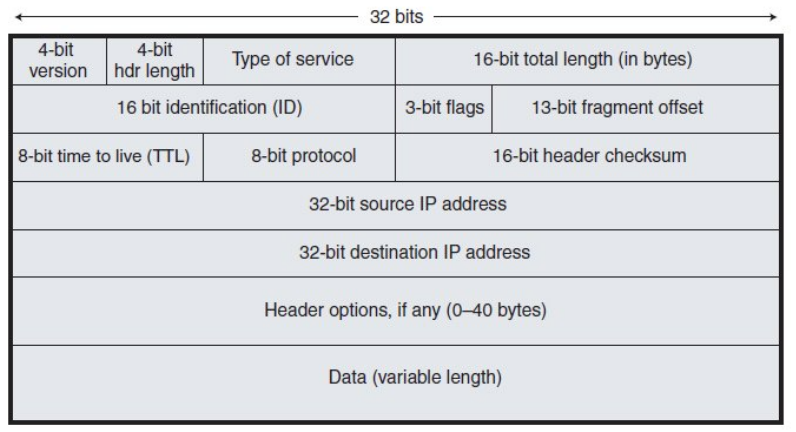
\includegraphics[width=\linewidth]{img/img09}
	\end{center}
\end{frame}

\section{Unicast, Broadcast and Multicast Traffic}

\begin{frame}
	\frametitle{Unicast, Broadcast and Multicast Traffic}
	\begin{itemize}
		\item There are 3 main IP traffic types: unicast, broadcast and multicast.
		\item Unicast traffic is to a single destination host.
		\item Broadcast traffic is to all hosts on the subnet.
		\item Multicast traffic is to multiple interested hosts.
	\end{itemize}
\end{frame}

\begin{frame}
	\frametitle{Unicast Traffic}
	\begin{center}
		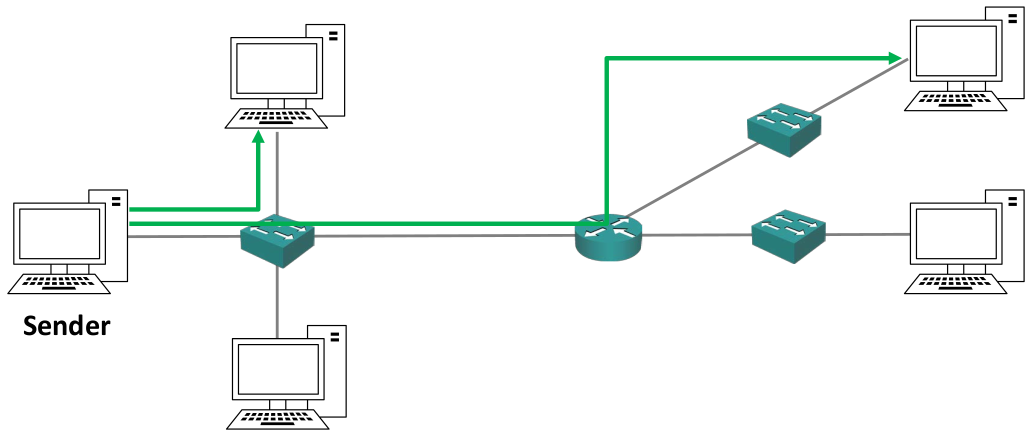
\includegraphics[width=\linewidth]{img/img10}
	\end{center}
\end{frame}

\begin{frame}
	\frametitle{Broadcast Traffic}
	\begin{center}
		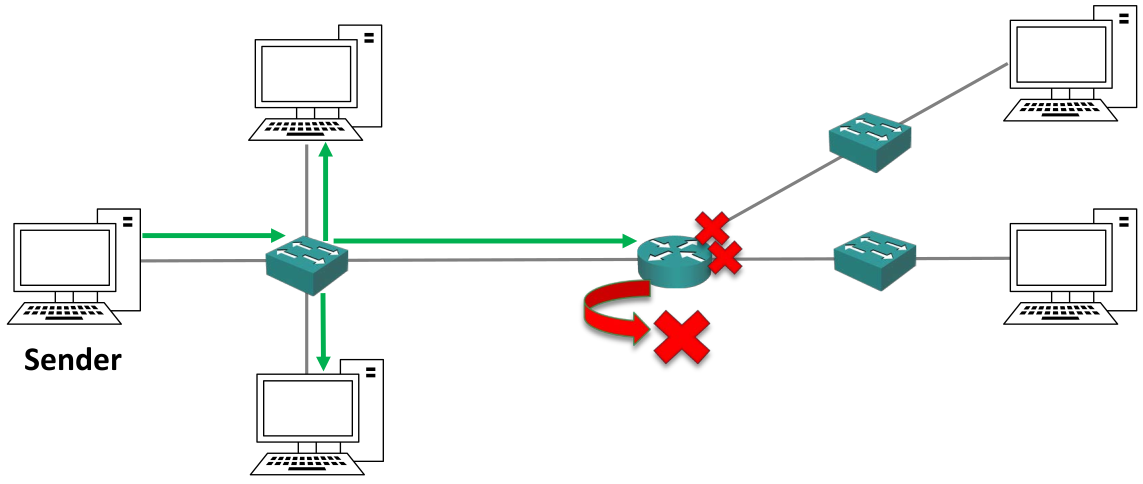
\includegraphics[width=\linewidth]{img/img11}
	\end{center}
\end{frame}

\begin{frame}
	\frametitle{Unicast Traffic to Multiple Hosts}
	\begin{center}
		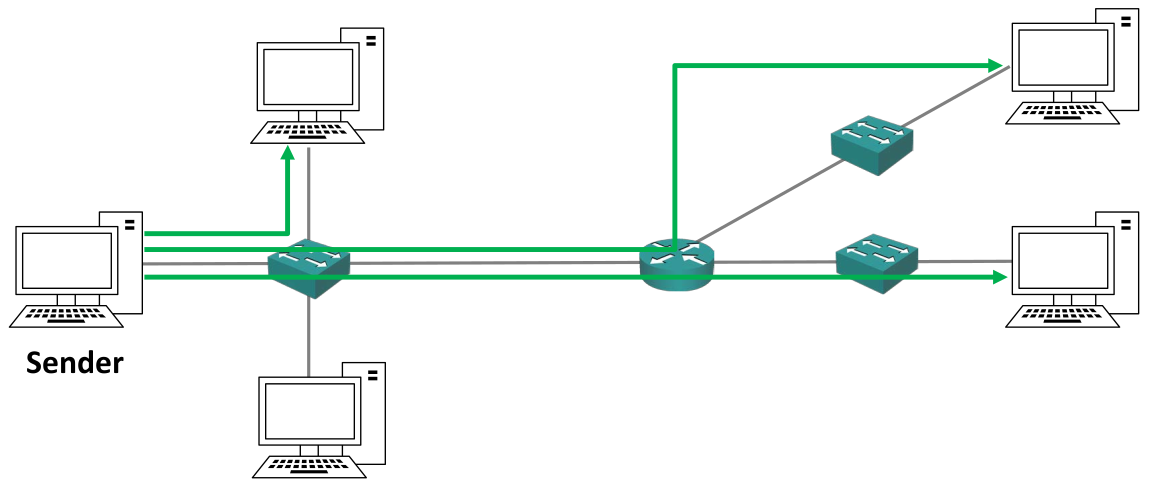
\includegraphics[width=\linewidth]{img/img12}
	\end{center}
\end{frame}

\begin{frame}
	\frametitle{Multicast Traffic}
	\begin{center}
		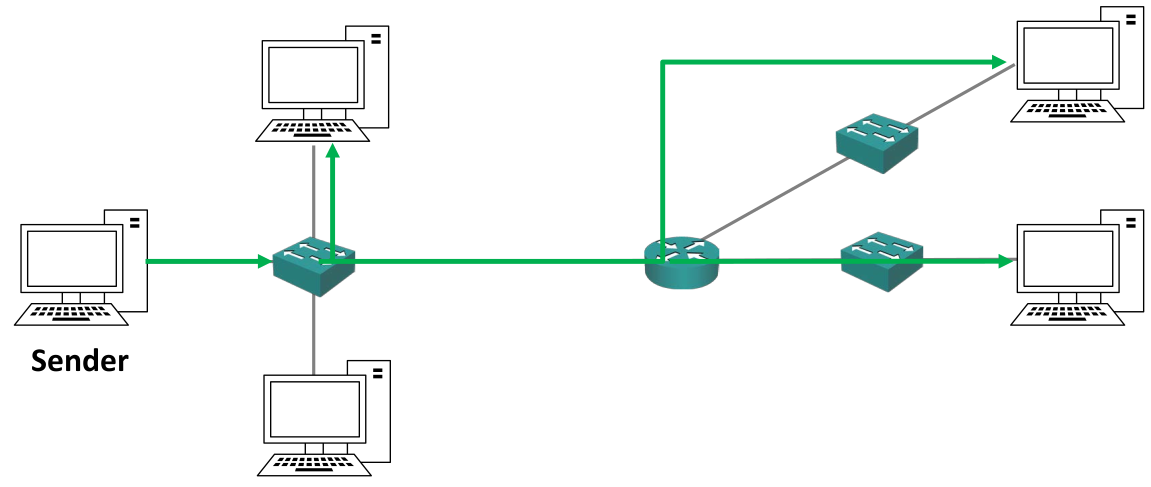
\includegraphics[width=\linewidth]{img/img13}
	\end{center}
\end{frame}

\section{Converting from Decimal to Binary}

\begin{frame}
	\frametitle{Counting in Decimal}
	\begin{itemize}
		\item Humans are conditioned to count in decimal.
		\item For each ‘column’ in a number we have 10 possible choices, from 0 to 9.
		\item Every time we add a column to the left, the value is multiplied by 10.
		\item We start with ‘1s’ as the furthest right column.
	\end{itemize}
	\begin{center}
		
\includegraphics[width=0.5\linewidth]{img/img14}
	\end{center}
\end{frame}

\begin{frame}
	\frametitle{Counting in Decimal}
	\begin{itemize}
		\item 236 is two 100’s, three 10’s, and six 1’s.
	\end{itemize}
	\begin{center}
		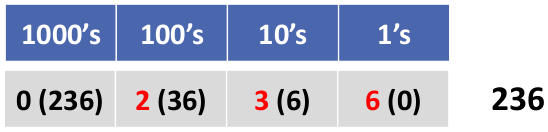
\includegraphics[width=0.6\linewidth]{img/img15}
	\end{center}
\end{frame}

\begin{frame}
	\frametitle{Counting in Binary}
	\begin{itemize}
		\item Computers work in binary.
		\item Electrical impulses are either off or on, so there’s only two choices (0 or 1), unlike 10 in decimal (0 to 9).
		\item For each ‘column’ in a number we have 2 possible choices, 0 or 1.
		\item Every time we add a column to the left, the value is multiplied by 2.
	\end{itemize}
	\begin{center}
		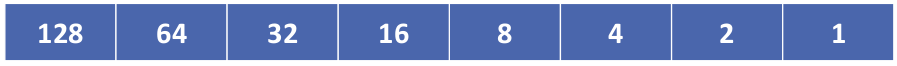
\includegraphics[width=0.8\linewidth]{img/img16}
	\end{center}
\end{frame}

\begin{frame}
	\frametitle{Counting in Binary}
	\begin{itemize}
		\item 236 in binary is 11101100
	\end{itemize}
	\begin{center}
		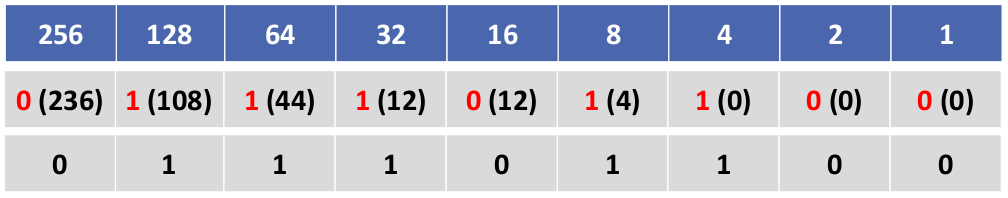
\includegraphics[width=0.9\linewidth]{img/img17}
	\end{center}
\end{frame}

\begin{frame}
	\frametitle{Counting in Binary}
	\begin{itemize}
		\item What is 179 in binary?
	\end{itemize}
	\begin{center}
		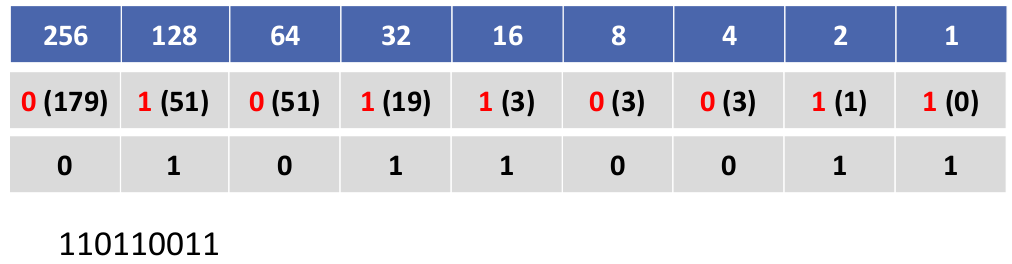
\includegraphics[width=0.9\linewidth]{img/img18}
	\end{center}
\end{frame}

\section{IPv4 Addresses}

\begin{frame}
	\frametitle{IPv4 Addresses}
	\begin{itemize}
		\item An IPv4 address is 32 bits long.
		\item It is written as 4 ‘octets’ in dotted decimal format.
		\item For example 192.168.10.15
		\item Each octet is 8 bits long $ (4 \times 8 = 32) $
	\end{itemize}	
\end{frame}



\end{document}